\chapter[EM Radiation]{Electromagnetic Radiation}
\label{p:em:emr12}

\section{Introduction}
This chapter will focus on the electromagnetic (EM) radiation. Electromagnetic radiation is a self-propagating wave in space with electric and magnetic components. These components oscillate at right angles to each other and to the direction of propagation, and are in phase with each other. Electromagnetic radiation is classified into types according to the frequency of the wave: these types include, in order of increasing frequency, radio waves, microwaves, infrared radiation, visible light, ultraviolet radiation, X-rays and gamma rays.

\chapterstartvideo{VPrsy}

\section{Particle/wave nature of electromagnetic radiation}
\label{p:em:emr12:d}
%\begin{syllabus}
%\item Explain that some aspects of the behaviour of EM radiation can best be explained using a wave model and some aspects can best be explained using a particle model
%\item Note: Link to Grade 12 Matter and Materials, photoelectric effect
%\end{syllabus}

\vspace{-0.5cm}

If you watch a colony of ants walking up the wall, they look like a thin continuous black line.  But as you look closer, you see that the line is made up of thousands of separated black ants.

Light and all other types of electromagnetic radiation seems like a continuous wave at first, but when one performs experiments with light, one can notice that light can have both wave and particle like properties.  Just like the individual ants, the light can also be made up of individual bundles of energy, or quanta of light.

Light has both wave-like and particle-like properties (wave--particle duality), but only shows one or the other, depending on the kind of experiment we perform. A wave-type experiment shows the wave nature, and a particle-type experiment shows particle nature.  One cannot test the wave and the particle nature at the same time. A particle of light is called a photon.

% \vspace{-2cm} % -0.5

\Definition{Photon}{A photon is a quantum (energy packet) of light.}

% \vspace{-0.1cm}

The particle nature of light can be demonstrated by the interaction of photons with matter.  One way in which light interacts with matter is via the photoelectric effect, which will be studied in detail in Chapter~\ref{p:mm:op12}.

\Exercise{Particle/wave nature of electromagnetic radiation}{
\begin{enumerate}[noitemsep]
\item Give examples of the behaviour of EM radiation which can best be explained using a wave model.
\item Give examples of the behaviour of EM radiation which can best be explained using a particle model.
\end{enumerate}
% Automatically inserted shortcodes - number to insert 2
\practiceinfo
\par \begin{tabular}[h]{cccccc}
% Question 1
(1.)	01m2	&
% Question 2
(2.)	01m3	&
\end{tabular}
% Automatically inserted shortcodes - number inserted 2
}

\section{The wave nature of electromagnetic radiation}
%\begin{syllabus}
%\item as mutual induction of oscillating magnetic/electric fields
%\item Describe the source of electromagnetic waves as an accelerating charge
%\item Use words and diagrams to explain how an EM wave propagates when an electric field oscillating in one plane produces a magnetic field oscillating in a plane at right angles to it, which produces an oscillating electric field, and so on  
%\item State that these mutually regenerating fields travel through space at a constant speed of 3x108m/s, represented by c.
%\item Note: Mention that unlike sound waves, EM waves do not need a medium to travel through
%\end{syllabus}

Accelerating charges emit electromagnetic waves. We have seen that a changing electric field generates a magnetic field and a changing magnetic field generates an electric field. This is the principle behind the propagation of electromagnetic waves, because electromagnetic waves, unlike sound waves, do not need a medium to travel through. EM waves propagate when an electric field oscillating in one plane produces a magnetic field oscillating in a plane at right angles to it, which produces an oscillating electric field, and so on. The propagation of electromagnetic waves can be described as \textit{mutual induction}. 

These mutually regenerating fields travel through empty space at a constant speed of $3 \times 10^8\ems$, represented by $c$.

\begin{center}
\scalebox{0.6}{% 0.8
\begin{pspicture}(-4,-4)(3,4)
\psset{Alpha=30}
\pstThreeDCoor[nameY=$B$,nameZ=$E$,linecolor=black,xMin=-4,yMin=-4,zMin=-4]
\parametricplotThreeD[xPlotpoints=200,linecolor=blue,linewidth=1.5pt,plotstyle=curve](-180,180){%
    t 60 div
    3 2.5 t mul cos mul
    0}
\parametricplotThreeD[xPlotpoints=200,linecolor=red,linewidth=1.5pt,plotstyle=curve](-180,180){%
    t 60 div
    0
     -3 2.5 t mul cos mul
    }
\end{pspicture}
}
\end{center}

%\begin{figure}[htp!]
%\nts{get this figure}%\includegraphics[width=0.75\textwidth]{../../epsimages/light-wave.eps}
%\label{ lightwave }
%\caption{ The propagation of electromagnetic waves }
%\end{figure}


\section{Electromagnetic spectrum}
\label{p:em:emr12:ems}

%\begin{syllabus}
%\item The learner given a list of different types of EM radiation, must be able to arrange them in order of frequency or wavelength.
%\item The learner Given the wavelength of EM waves, must be able to calculate the frequency and vice versa, using the equation c=f.lambda.
%\item The learner must be able to Give an example of the use of each type of EM radiation, i.e.\@ gamma rays, X-rays, ultraviolet light, visible light, infrared, microwave and radio and TV waves.
%\item Note: Link to Grade 10 Waves, Sound and Light
%\end{syllabus}



\begin{figure}[htbp]
\begin{center}
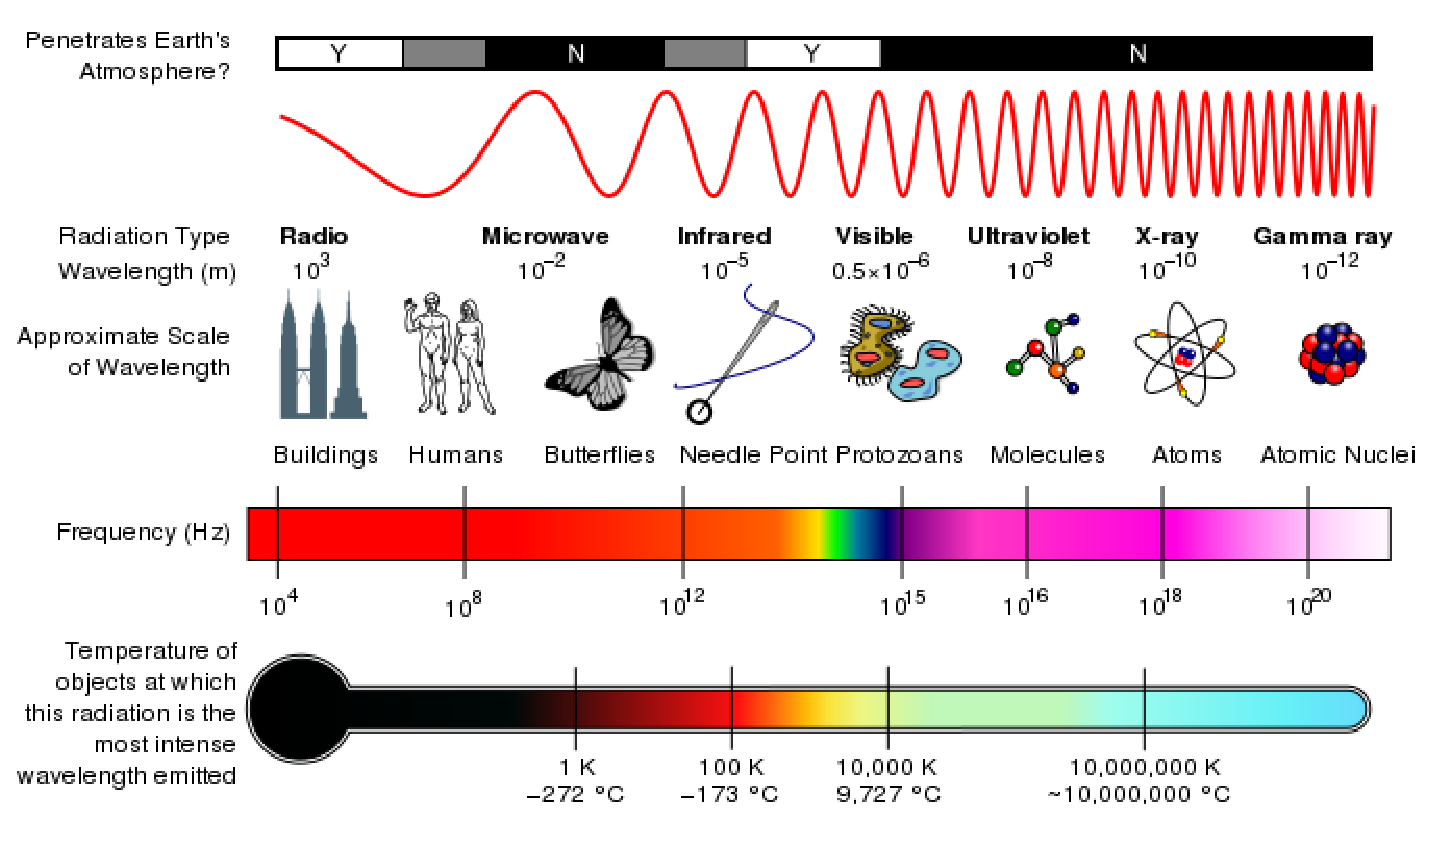
\includegraphics[width=0.95\textwidth]{../../epsimages/EM_Spectrum_Properties_edit.eps}%very big so leave out for now s}
\caption{The electromagnetic spectrum as a function of frequency. The different types according to wavelength are shown as well as everyday comparisons.}
\end{center}
\end{figure}

Observe the things around you, your friend sitting next to you, a large tree across the field. How is it that you are able to see these things? What is it that is leaving your friend's arm and entering your eye so that you can see his arm? It is light. The light originally comes from the sun, or possibly a light bulb or burning fire. In physics, light is given the more technical term electromagnetic radiation, which includes all forms of light, not just the form which you can see with your eyes. 

Electromagnetic radiation allows us to observe the world around us. It is this radiation which reflects off of the objects around you and into your eye. The radiation your eye is sensitive to is only a small fraction of the total radiation emitted in the physical universe. All of the different fractions taped together make up the electromagnetic spectrum. 

\Extension{Dispersion}{When white light is split into its component colours by a prism, you are looking at a portion of the electromagnetic spectrum.}

The wavelength of a particular electromagnetic radiation will depend on how it was created. 

\clearpage

\Exercise{Wave Nature of EM Radiation}{
\begin{enumerate}
\item List one source of electromagnetic waves. Hint: consider the spectrum diagram and look at the names we give to different wavelengths.
\item Explain how an EM wave propagates, with the aid of a diagram.
\item What is the speed of light? What symbol is used to refer to the speed of light? Does the speed of light change?
\item Do EM waves need a medium to travel through? 
\end{enumerate}

% Automatically inserted shortcodes - number to insert 4
\vspace{-0.5cm}
\par \practiceinfo
\vspace{-0.5cm}
\par \begin{tabular}[h]{cccccc}
% Question 1
(1.)	01m4	&
% Question 2
(2.)	01m5	&
% Question 3
(3.)	01m6	&
% Question 4
(4.)	01m7	&
\end{tabular}
% Automatically inserted shortcodes - number inserted 4
}

The radiation can take on any wavelength, which means that the spectrum is continuous. Physicists broke down this continuous band into sections. Each section is defined by how the radiation is created, not the wavelength of the radiation. But each category is continuous within the min and max wavelength of that category, meaning there are no wavelengths excluded within some range. 

The spectrum is in order of wavelength, with the shortest wavelength at one end and the longest wavelength at the other. The spectrum is then broken down into categories as detailed in Table~\ref{tab:emspectrum}.

\begin{table}[H]
\begin{center}
\caption{Electromagnetic spectrum}
\label{tab:emspectrum}
\begin{tabular}{|c|c|c|}\hline
\textbf{Category}&\textbf{Range of Wavelengths (nm)}&\textbf{Range of Frequencies (Hz)}\\\hline\hline
gamma rays&$<$1&$>3\times 10^{19}$ \\\hline
X-rays&1-10&$3\times 10^{17}$-$3\times 10^{19}$\\\hline
ultraviolet light&10-400&$7,5\times 10^{14}$-$3\times 10^{17}$\\\hline
visible light&400-700&$4,3\times 10^{14}$-$7,5\times 10^{14}$\\\hline
infrared&700-$10^{5}$&$3\times 10^{12}$-$4,3\times 10^{19}$\\\hline
microwave&$10^{5}-10^{8}$&$3\times 10^{9}$-$3\times 10^{12}$\\\hline
radio waves&$>10^{8}$&$<3\times 10^{9}$\\\hline
\end{tabular}
\end{center}
\end{table}

Since an electromagnetic wave is still a wave, the equation that you learnt in Grade 10 still applies:
$c=f\cdot \lambda$.

\clearpage

\begin{wex}{EM spectrum I}{Calculate the frequency of red light with a wavelength of $4,2 \times 10^{-7}$~m}{ 
We use the formula: $c=f\lambda$ to calculate frequency. The speed of light is a constant $3 \times 10^{8}$m/s.
\begin{eqnarray*}
c&=&f\lambda\\
3 \times 10^{8}&=&f \times 4,2 \times 10^{-7} \\
f &=& 7,14 \times 10^{14} \rm {Hz}
\end{eqnarray*}}
\end{wex}

\begin{wex}{EM spectrum II}
{Ultraviolet radiation has a wavelength of $200~\mathrm{nm}$. What is the frequency of the radiation?}
{\westep{To calculate the frequency we need to identify the
wavelength and the velocity of the radiation.}
Recall that all radiation travels at the speed of light ($c$) in vacuum.
Since the question does not specify through what type of material the Ultraviolet radiation
is travelling, one can assume that it is travelling through a vacuum.
We can identify two properties of the radiation - $wavelength
~(200~\mathrm{nm})$ and speed ($c$).
%From previous chapters, we know that the period of the wave
%is the time it takes
%for a wave to complete one cycle or one wavelength. 

\westep{We can use the equation $c = f \lambda$ to find the frequency since the wavelength is given.}
\begin{eqnarray*}
c &=& f \lambda \\
3 \times 10^{8} &=& f \times 200 \times 10^{-9} \\
f &=&  1.5 \times 10^{15} \ \rm{Hz}
\end{eqnarray*}
}
\end{wex}

Examples of some uses of electromagnetic waves are shown in Table~\ref{tab:emuses}. 

\begin{table}[htbp]
\begin{center}
\caption{Uses of EM waves}
\label{tab:emuses}
\begin{tabular}{|c|p{5cm}|}\hline
\textbf{Category}&\textbf{Uses}\\\hline\hline
gamma rays&used to kill the bacteria in marshmallows and to sterilise medical equipment\\\hline
X-rays&used to image bone structures\\\hline
ultraviolet light&bees can see into the ultraviolet because flowers stand out more clearly at this frequency\\\hline
visible light&used by humans to observe the world\\\hline
infrared&night vision, heat sensors, laser metal cutting\\\hline
microwave&microwave ovens, radar\\\hline
radio waves&radio, television broadcasts\\\hline
\end{tabular}
\end{center}
\end{table}

In theory the spectrum is infinite, although realistically we can only observe wavelengths from a few hundred kilometres to those of gamma rays due to experimental limitations. 

Humans experience electromagnetic waves differently depending on their wavelength. Our eyes are sensitive to visible light while our skin is sensitive to infrared, and many wavelengths we do not detect at all.

\Exercise{EM Radiation}
{
\begin{enumerate}
\item Arrange the following types of EM radiation in order of increasing frequency: infrared, X-rays, ultraviolet, visible, gamma. 
\item Calculate the frequency of an EM wave with a wavelength of 400~nm.
\item Give an example of the use of each type of EM radiation: gamma rays, X-rays, ultraviolet light, visible light, infrared, microwave and radio and TV waves.
\end{enumerate}

% Automatically inserted shortcodes - number to insert 3
\vspace{-0.75cm}
\par \practiceinfo
\vspace{-0.5cm}
\par \begin{tabular}[h]{cccccc}
% Question 1
(1.)	01m8	&
% Question 2
(2.)	01m9	&
% Question 3
(3.)	01ma	&
\end{tabular}
% Automatically inserted shortcodes - number inserted 3
}

\clearpage

\section{The particle nature of electromagnetic radiation}
%\begin{syllabus}
%\item energy of a photon related to frequency and wavelength
%\item Calculate the energy of a photon using E = hf = hc/lambda
%\end{syllabus}

When we talk of electromagnetic radiation as a particle, we refer to photons, which are packets of energy. The energy of the photon is related to the wavelength of electromagnetic radiation according to:
%\equ{E=h\cdot f= \frac{hc}{\lambda}}{eq:ehf}
$h$ (called Planck's constant).

\vspace{-0.5cm}

\Definition{Planck's constant}{Planck's constant is a physical constant named after Max Planck.

\nequ{h =6,626 \times 10^{-34}\ \mbox{J}\cdot\mbox{s}}
}

The energy of a photon can be calculated using the formula: $E=hf$ or $E=h \frac{c}{\lambda}$.
Where E is the energy of the photon in joules (J), h is Planck's constant, c is the speed of light, f is the frequency in hertz (Hz) and $\lambda$ is the wavelength in metres (m).

\begin{wex}{Calculating the energy of a photon I}{Calculate the energy of a photon with a frequency of $3 \times 10^{18}$~Hz}
{We use the formula:
\begin{eqnarray*}
E &=& hf\\
&=& 6,6 \times 10^{-34} \times 3 \times 10^{18}\\
&=& 2 \times 10^{-15} \eJ\\
\end{eqnarray*}}
\end{wex}

\begin{wex}{Calculating the energy of a photon II}
{What is the energy of an ultraviolet photon with a wavelength of 200~nm?}
{\westep{Determine what is required and how to approach the problem.}
We are required to calculate the energy associated with a photon of ultraviolet light with a wavelength of  200~nm.

We can use:
\nequ{E=h\frac{c}{\lambda}}

\westep{Solve the problem}
\begin{eqnarray*}
E & = & h\frac{c}{\lambda}\\
& = & (6,626 \times 10^{-34})\frac{3\times10^{8}}{200\times 10^{-9}}\\
& = & 9,939 \times 10^{-10}\eJ
\end{eqnarray*}}
\end{wex}


\Exercise{particle nature of EM waves}{
\begin{enumerate}
\item How is the energy of a photon related to its frequency and wavelength?
\item Calculate the energy of a photon of EM radiation with a frequency of $10^{12}$~Hz.
\item Determine the energy of a photon of EM radiation with a wavelength of 600 nm.
\end{enumerate}
% Automatically inserted shortcodes - number to insert 3
\par \practiceinfo
\par \begin{tabular}[h]{cccccc}
% Question 1
(1.)	01z3	&
% Question 2
(2.)	01z4	&
% Question 3
(3.)	01z5	&
\end{tabular}
% Automatically inserted shortcodes - number inserted 3
}

\section{Penetrating ability of electromagnetic radiation}
\label{p:em:emr12:pa}
%\begin{syllabus}
%\item Indicate the penetrating ability of the different kinds of EM radiation and relate it to energy of the radiation.
%\item Describe the dangers of gamma rays, X-rays and the damaging effect of ultra-violet radiation on skin
%\item Note: Link to Grade 11 Matter and Materials, atomic nuclei
%\end{syllabus}

Different kinds of electromagnetic radiation have different penetrabilities. For example, if we take the human body as the object. Infrared light is emitted by the human body. Visible light is reflected off the surface of the human body, ultra-violet light (from sunlight) damages the skin, but X-rays are able to penetrate the skin and bone and allow for pictures of the inside of the human body to be taken.

If we compare the energy of visible light to the energy of X-rays, we find that X-rays have a much higher energy. Usually, kinds of electromagnetic radiation with higher energy have higher penetrabilities than those with low energies.

Certain kinds of electromagnetic radiation such as ultra-violet radiation, X-rays and gamma rays are very dangerous. Radiation such as these are called ionising radiation. Ionising radiation transfers energy as it passes through matter, breaking molecular bonds and creating ions.
 
Excessive exposure to radiation, including sunlight, X-rays and all nuclear radiation, can cause destruction of biological tissue. 

\vspace{-0.5cm}

\subsection{Ultraviolet (UV) radiation and the skin}
UVA and UVB are different ranges of frequencies for ultraviolet (UV) light. UVA and UVB can damage collagen fibres which results in the speeding up skin ageing. In general, UVA is the least harmful, but it  can contribute to the ageing of skin, DNA damage and possibly skin cancer. It penetrates deeply and does not cause sunburn. Because it does not cause reddening of the skin (erythema) it cannot be measured in the SPF testing. There is no good clinical measurement of the blocking of UVA radiation, but it is important that sunscreen block both UVA and UVB.

UVB light can cause skin cancer. The radiation excites DNA molecules in skin cells, resulting in possible mutations, which can cause cancer. This cancer connection is one reason for concern about ozone depletion and the ozone hole.

As a defence against UV radiation, the body tans when exposed to moderate (depending on skin type) levels of radiation by releasing the brown pigment melanin. This helps to block UV penetration and prevent damage to the vulnerable skin tissues deeper down. Suntan lotion, often referred to as sunblock or sunscreen, partly blocks UV and is widely available. Most of these products contain an SPF rating that describes the amount of protection given. This protection, however, applies only to UVB rays responsible for sunburn and not to UVA rays that penetrate more deeply into the skin and may also be responsible for causing cancer and wrinkles. Some sunscreen lotion now includes compounds such as titanium dioxide which helps protect against UVA rays. Other UVA blocking compounds found in sunscreen include zinc oxide and avobenzone.

%\Extension{What makes a good sunscreen?}{\begin{itemize}
%\item UVB protection: Padimate O, Homosalate, Octisalate (octyl salicylate), Octinoxate (octyl methoxycinnamate)
%\item UVA protection: Avobenzone
%\item UVA/UVB protection: Octocrylene, titanium dioxide, zinc oxide, Mexoryl (ecamsule)
%\end{itemize}
%Another means to block UV is by wearing sun protective clothing. This is clothing that has a UPF rating that describes the protection given against both UVA and UVB.}

\subsection{Ultraviolet radiation and the eyes}
High intensities of UVB light are hazardous to the eyes, and exposure can cause welder's flash (photo keratitis or arc eye) and may lead to cataracts, pterygium and pinguecula formation.

Protective eyewear is beneficial to those who are working with or those who might be exposed to ultraviolet radiation, particularly short wave UV. Given that light may reach the eye from the sides, full coverage eye protection is usually warranted if there is an increased risk of exposure, as in high altitude mountaineering. Mountaineers are exposed to higher than ordinary levels of UV radiation, both because there is less atmospheric filtering and because of reflection from snow and ice.

Ordinary, untreated eyeglasses give some protection. Most plastic lenses give more protection than glass lenses. Some plastic lens materials, such as polycarbonate, block most UV. There are protective treatments available for eyeglass lenses that need it which will give better protection. But even a treatment that completely blocks UV will not protect the eye from light that arrives around the lens. To convince yourself of the potential dangers of stray UV light, cover your lenses with something opaque, like aluminium foil, stand next to a bright light, and consider how much light you see, despite the complete blockage of the lenses. Most contact lenses help to protect the retina by absorbing UV radiation.

\subsection{X-rays}
While x-rays are used significantly in medicine, prolonged exposure to X-rays can lead to cell damage and cancer.

For example, a mammogram is an x-ray of the human breast to detect breast cancer, but if a woman starts having regular mammograms when she is too young, her chances of getting breast cancer increases.

\subsection{Gamma-rays}
Due to the high energy of gamma-rays, they are able to cause serious damage when absorbed by living cells.

Gamma-rays are not stopped by the skin and can induce DNA alteration by interfering with the genetic material of the cell. DNA double-strand breaks are generally accepted to be the most biologically significant lesion by which ionising radiation causes cancer and hereditary disease.

A study done on Russian nuclear workers exposed to external whole-body gamma-radiation at high cumulative doses shows a link between radiation exposure and death from leukaemia, lung, liver, skeletal and other solid cancers.


\Extension{Cellphones and electromagnetic radiation}{Cellphone radiation and health concerns have been raised, especially following the enormous increase in the use of wireless mobile telephony throughout the world. This is because mobile phones use electromagnetic waves in the microwave range. These concerns have induced a large body of research. Concerns about effects on health have also been raised regarding other digital wireless systems, such as data communication networks.
In 2009 the World Health Organisation announced that they have found a link between brain cancer and cellphones.

Cellphone users are recommended to minimise radiation, by for example:

\begin{enumerate}
\item Use hands-free to decrease the radiation to the head.
\item Keep the mobile phone away from the body.
\item Do not telephone in a car without an external antenna.
\end{enumerate}

}

\Exercise{}{
\begin{enumerate}
\item Indicate the penetrating ability of the different kinds of EM radiation and relate it to energy of the radiation.
\item Describe the dangers of gamma rays, X-rays and the damaging effect of ultra-violet radiation on skin
\end{enumerate}

% Automatically inserted shortcodes - number to insert 2
\par \practiceinfo
\par \begin{tabular}[h]{cccccc}
% Question 1
(1.)	01mb	&
% Question 2
(2.)	01mc	&
\end{tabular}
% Automatically inserted shortcodes - number inserted 2

}
% Presentation on the electromagnetic spectrum: SIYAVULA-PRESENTATION:http://cnx.org/content/m39513/latest/#slidesharefigure

\clearpage

\summary{VPpxh}
\begin{itemize}
\item Electromagnetic radiation has both a wave and a particle nature.
\item Electromagnetic waves travel at a speed of $3 \times 10^{8}~m \cdot s^{-1}$ in a vacuum.
\item The Electromagnetic spectrum consists of the following types of radiation: radio waves, microwaves, infrared, visible, ultraviolet, X-rays, gamma-rays.
\item Gamma-rays have the most energy and are the most penetrating, while radio waves have the lowest energy and are the least penetrating.
\end{itemize}

\begin{eocexercises}{}
\begin{enumerate}

\item What is the energy of a photon of EM radiation with a frequency of $3 \times 10^{8}$~Hz? 

\item What is the energy of a photon of light with a wavelength of 660~nm?

\item List the main types of electromagnetic radiation in order of increasing wavelength.

\item List the main uses of:
\begin{enumerate}
\item radio waves
\item infrared
\item gamma rays
\item X-rays
\end{enumerate}

\item Explain why we need to protect ourselves from ultraviolet radiation from the Sun.

\item List some advantages and disadvantages of using X-rays.

\item What precautions should we take when using cell phones?

\item Write a short essay on a type of electromagnetic wave. You should look at uses, advantages and disadvantages of the radiation.

\item Explain why some types of electromagnetic radiation are more penetrating than others.

\end{enumerate}

% Automatically inserted shortcodes - number to insert 9
\par \practiceinfo
\par \begin{tabular}[h]{cccccc}
% Question 1
(1.)	01md	&
% Question 2
(2.)	01me	&
% Question 3
(3.)	01mf	&
% Question 4
(4.)	01mg	&
% Question 5
(5.)	01mh	&
% Question 6
(6.)	01mi	\\ % End row of shortcodes
% Question 7
(7.)	01mj	&
% Question 8
(8.)	01mk	&
% Question 9
(9.)	01mm	&
\end{tabular}
% Automatically inserted shortcodes - number inserted 9

\end{eocexercises}



% CHILD SECTION END 



% CHILD SECTION START 

